% !TeX spellcheck = en_EN-English

\chapter{Medical data} \label{chap:data}

\mycomment{
EQUATION SHOWCASE:
\begin{equation}
	\label{eqn:starskynoise}
	\sigma_{star} = \sqrt{S_{star}} \quad \sigma_{sky} = \sqrt{S_{sky}}
\end{equation} 

FIGURE SHOWCASE:
\begin{figure}[!h]
	\centering
	\begin{subfigure}{.3\textwidth}
		\centering
		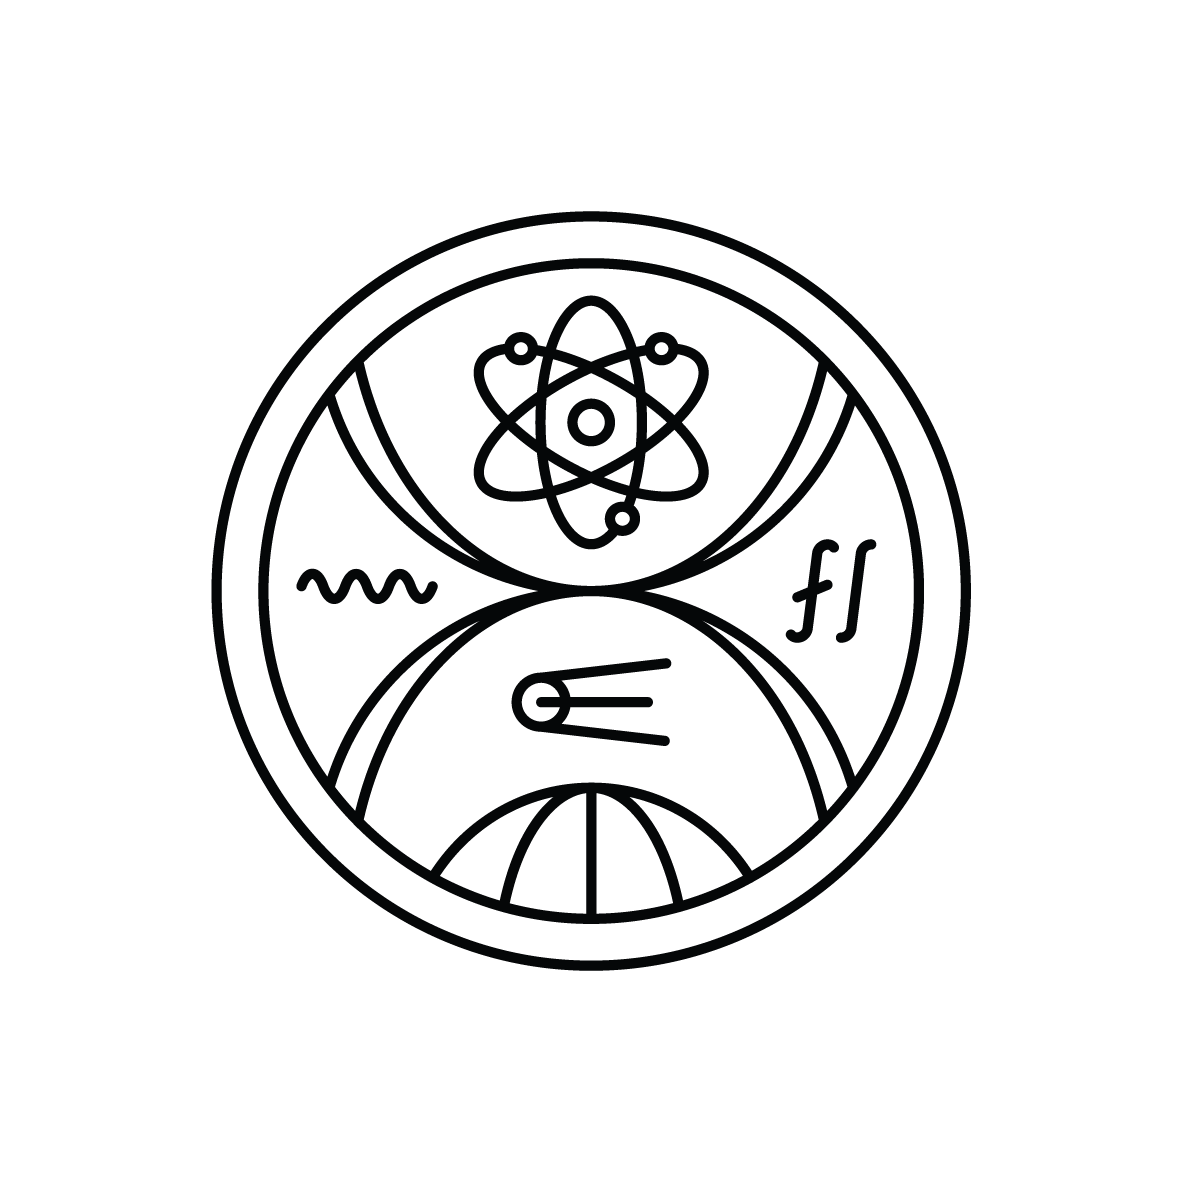
\includegraphics[width=\textwidth]{images/FMFI_logo_BP.png}
		\caption{Hot pixels.}
		\label{fig:hotpixels}
	\end{subfigure}
	\begin{subfigure}{.3\textwidth}
		\centering
		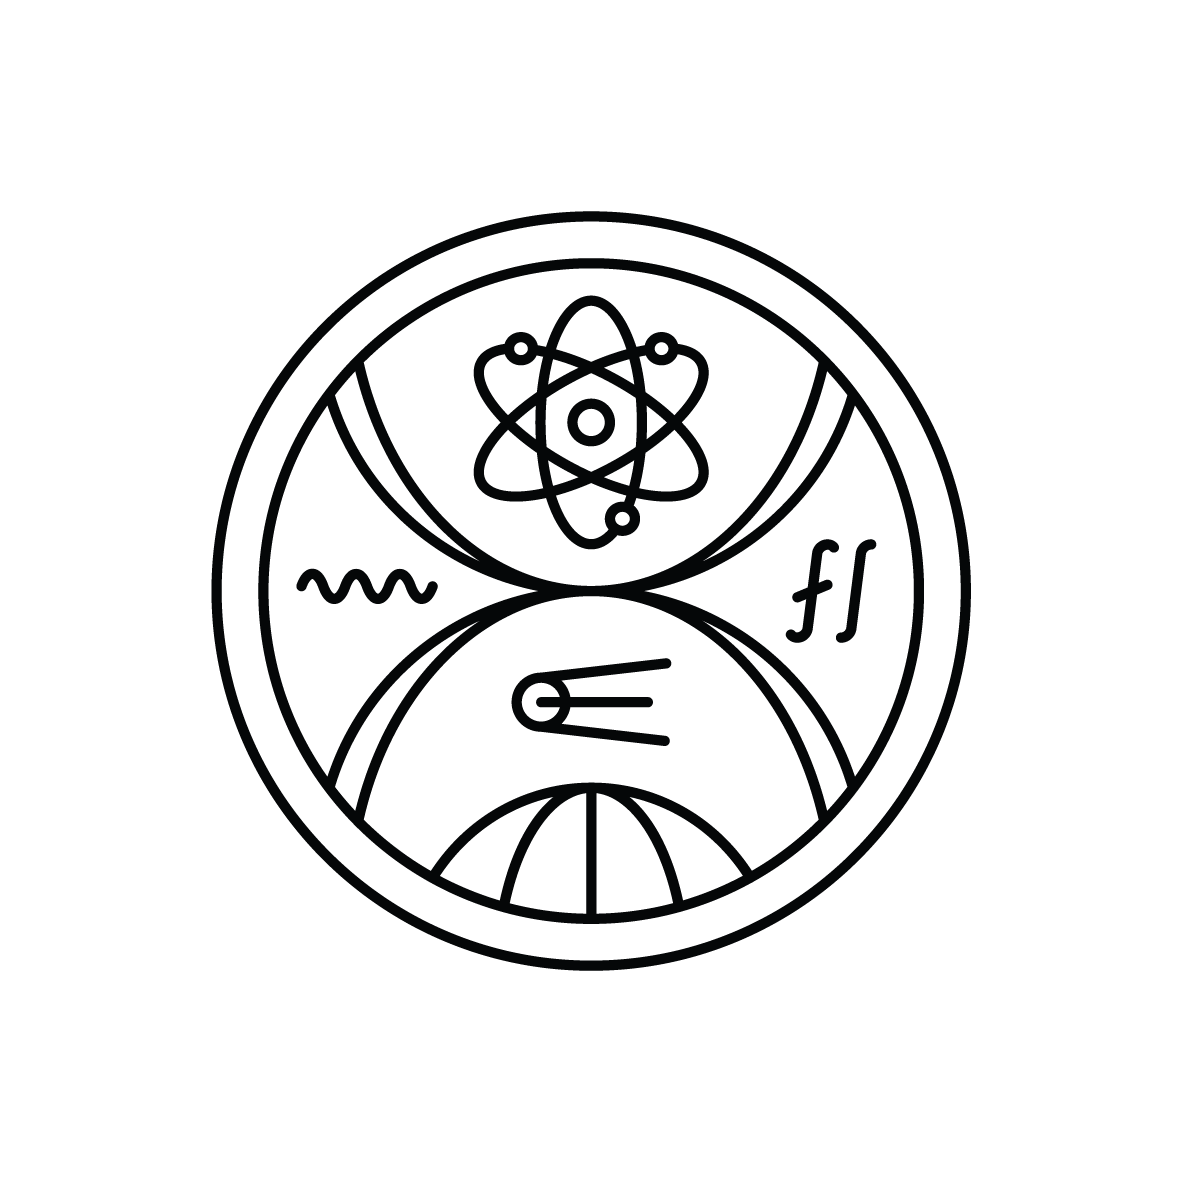
\includegraphics[width=\textwidth]{images/FMFI_logo_BP.png}
		\caption{Dead columns.}
		\label{fig:deadcolumns}
	\end{subfigure}
	
	\vspace*{4mm}
	
	\begin{subfigure}{.3\textwidth}
		\centering
		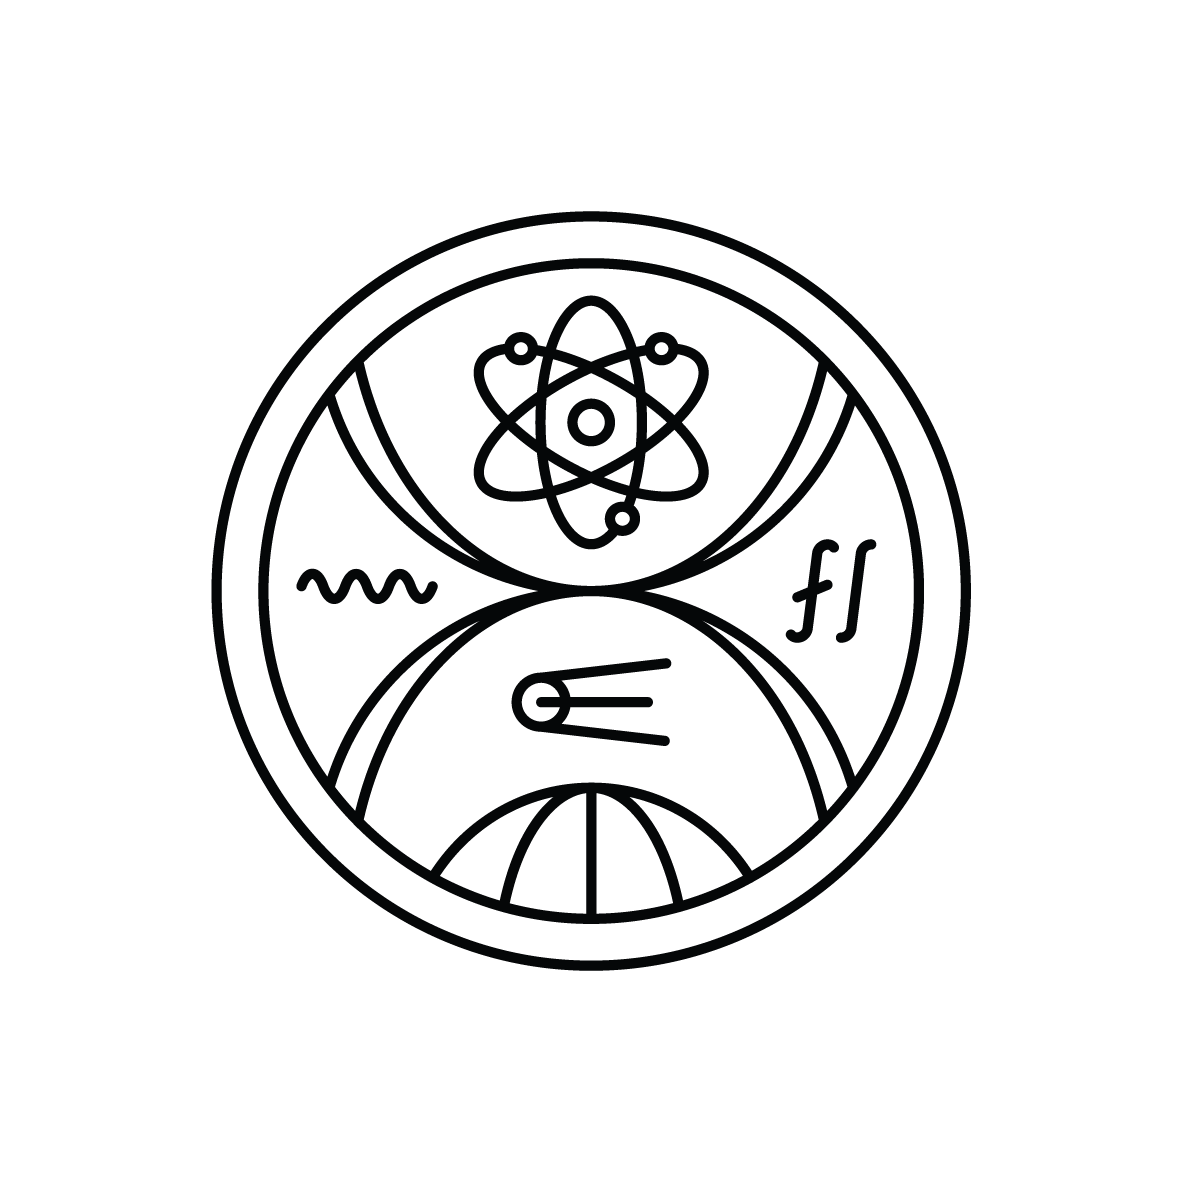
\includegraphics[width=\textwidth]{images/FMFI_logo_BP.png}
		\caption{Traps.}
		\label{fig:trap}
	\end{subfigure}
	\begin{subfigure}{.3\textwidth}
		\centering
		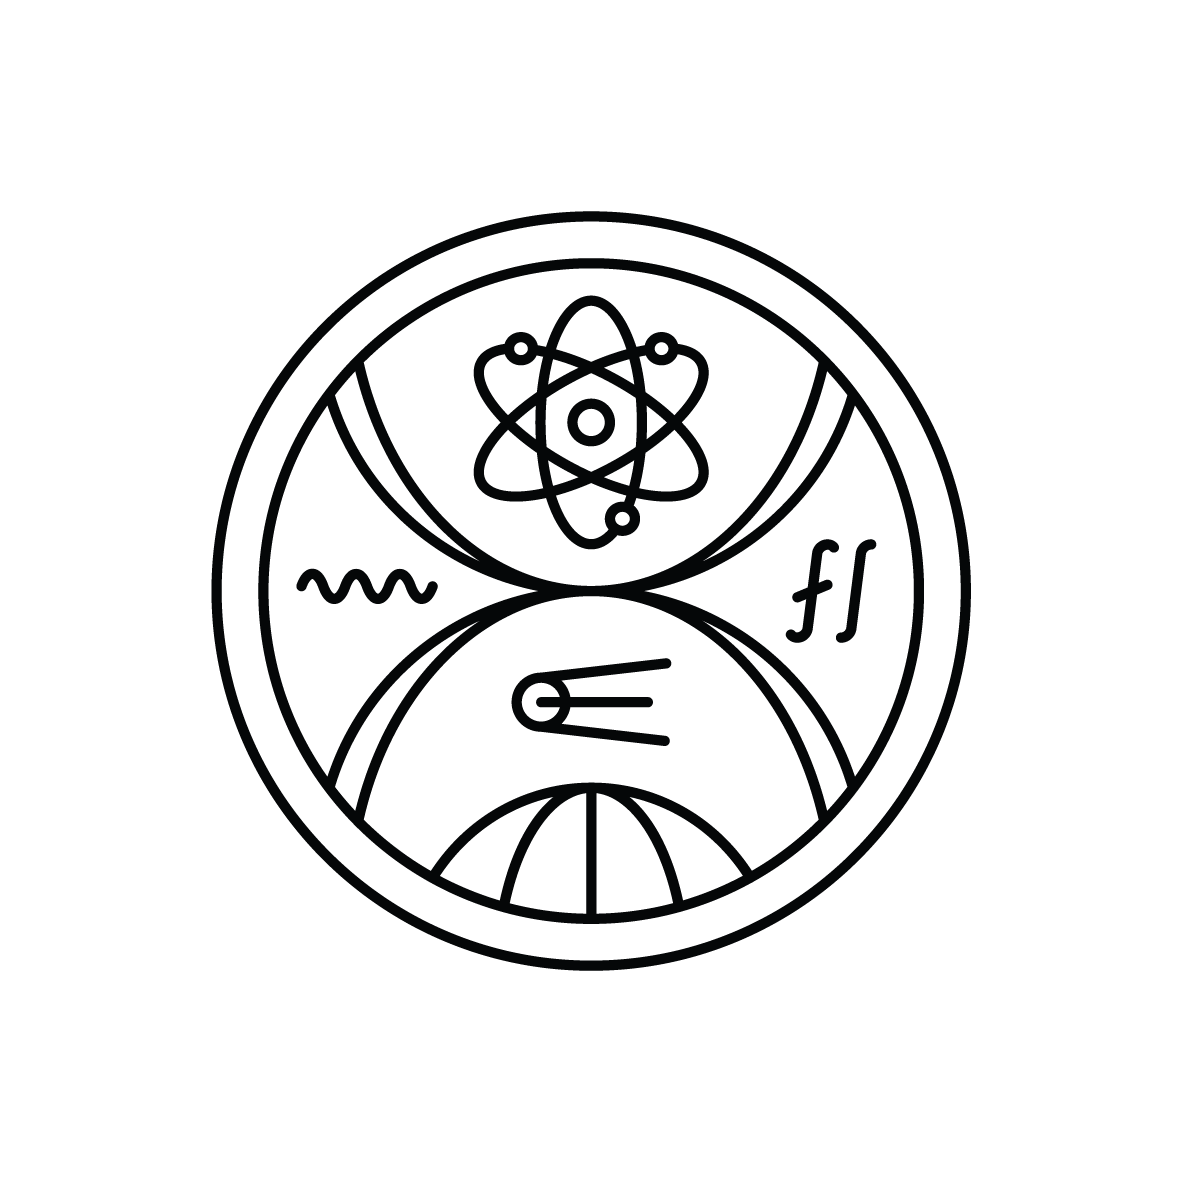
\includegraphics[width=\textwidth]{images/FMFI_logo_BP.png}
		\caption{Saturation trail.}
		\label{fig:saturationtrail}
	\end{subfigure}
	\caption{Examples of some internal defects present on FITS images acquired by AGO70.}
	\label{fig:internaldefects}
\end{figure}
}